% Provenance (never printed): see sources/outline_sources.md (Year 3:
% fractionation and Rayleigh distillation in the water cycle;
% palaeothermometry; carbon and sulfur isotopes). Brief:
% sources/book5/BRIEFS.md, ch. 14. Curves from figdata/bachelor-3/
% rayleigh_distillation.py, lr04_d18o.py, carbon_mass_balance.py. Exercise
% and problem values in the Book 5 scratch calculator calc/ch14.py. Dome Ilse,
% its traverse and the marine core are invented.
\chapter{Stable-Isotope Geochemistry}\label{ch:b3:stable-isotopes}

Snow falling on the high domes of the East Antarctic ice sheet is among the
lightest water on Earth. Each of its molecules left the ocean as vapour, and
on the way inland the air lost most of its water as snow, the heavy molecules
first. What is left on arrival depends on how much was lost, which depends on
how cold the air became. A column of ice is therefore a thermometer, a shell
of calcite another, and the carbon of limestones a ledger of what the
biosphere buried. This chapter derives the laws behind these records and
reads them.

\begin{recall}
The $\delta$ value, the fractionation factor $\alpha$ and the equilibrium and
kinetic isotope effects are in the chemistry books' university volumes. The
reference standards VSMOW and VPDB and the meteoric water line are in the
Year 2 volume, in its chapter on isotope geochemistry; the Rayleigh
fractionation law of trace elements in its chapter on magmatic
differentiation; climate proxies, the ice-volume effect and the Mg/Ca
thermometer in its chapter on climate archives and proxies; the
Palaeocene--Eocene Thermal Maximum in its chapter on climate over geological
time; the Great Oxidation Event in its chapter on the Precambrian Earth.
Photosynthesis and bacterial sulfate reduction are in the biology books.
\end{recall}

\section{Fractionation between two phases}\label{sec:b3:stable-isotopes:fractionation}

For two phases A and B in isotopic equilibrium, $\alpha_{A-B} = R_A/R_B =
(1000 + \delta_A)/(1000 + \delta_B)$, with the ratios $R$ of the heavy to the
light isotope. Water vapour and liquid water have $\alpha = 1.0098$ for oxygen-18
and $1.084$ for deuterium at \qty{20}{\celsius}, $1.0117$ and $1.111$ at
\qty{0}{\celsius}; ice and water at \qty{0}{\celsius}, $1.0035$ and $1.0208$.
The heavier phase is always the more condensed one, and the fractionation
grows as the temperature falls.
% ledger: kc98:alpha, kc98:standards

\begin{definition}[Isotopic difference]\label{def:b3:stable-isotopes:big-delta}
The \emph{isotopic difference}\index{isotopic difference (capital delta)}
between two phases is $\Delta_{A-B} = \delta_A - \delta_B$, in per mil.
\end{definition}

\begin{proposition}[The isotopic difference and the fractionation factor]
\label{prop:b3:stable-isotopes:big-delta}
For $\alpha$ close to 1 and small $\delta$ values,
\[
\Delta_{A-B} \approx 1000\ln\alpha_{A-B} \approx 1000(\alpha_{A-B} - 1).
\]
\end{proposition}

\begin{proof}
$1000\ln\alpha = 1000\ln(1 + \delta_A/1000) - 1000\ln(1 + \delta_B/1000)$, and
$1000\ln(1 + x/1000) = x - x^2/2000 + \dots$, so $1000\ln\alpha = \delta_A -
\delta_B - (\delta_A^2 - \delta_B^2)/2000 + \dots$. Finally $\ln\alpha \approx
\alpha - 1$ for $\alpha$ near 1.
\end{proof}

The error is $(\delta_A^2 - \delta_B^2)/2000$: a fraction of a per mil at the
values of the ocean, nearly a per mil between the ocean and the light snow of
polar ice.
The quantity $1000\ln\alpha$ is the one that theory relates to temperature: it
varies nearly as $1/T^2$ at high temperature and as $1/T$ at low temperature,
and calibrations are written in that form. For ice and vapour, for instance,
\[
\ln\alpha^{18}_{\mathrm{ice-v}} = \frac{11.839}{T} - 0.028224, \qquad
\ln\alpha^{\mathrm D}_{\mathrm{ice-v}} = \frac{16288}{T^2} - 0.0934,
\]
with $T$ in kelvins.
% ledger: gkinis14:alpha-ice, kc98:standards

\begin{definition}[Mass-dependent and mass-independent fractionation]\label{def:b3:stable-isotopes:mif}
An element with three isotopes or more has a \emph{mass-dependent
fractionation}\index{mass-dependent fractionation} when the fractionations of
its isotope ratios are in the ratio of their mass differences, as set by the
masses; otherwise it has a \emph{mass-independent
fractionation}\index{mass-independent fractionation}, measured by the departure
from the mass-dependent line, such as $\Delta^{33}\mathrm S = \delta^{33}\mathrm S
- 0.515\,\delta^{34}\mathrm S$.
\end{definition}

For oxygen, the fractionation of $^{17}\mathrm O/^{16}\mathrm O$ is about 0.52 times that
of $^{18}\mathrm O/^{16}\mathrm O$, close to the ratio of the mass differences, 1 to 2;
for sulfur, $\delta^{33}\mathrm S = 0.515\,\delta^{34}\mathrm S$. \omterm{def:b3:stable-isotopes:mif}{Mass-independent
fractionation} is rare: it is found in meteorites, in stratospheric ozone and
in Archean sulfur.
% ledger: white13c9:mdf, white13c9:s-mif

\section{Rayleigh distillation in the water cycle}\label{sec:b3:stable-isotopes:rayleigh}

An air mass that cools makes cloud droplets or snow crystals, which fall and
leave. Each condensate is richer in the heavy isotopes than the vapour, so the
vapour left grows lighter, and the next condensate, in equilibrium with it, is
lighter too.

\begin{proposition}[Rayleigh distillation]\label{prop:b3:stable-isotopes:rayleigh-distillation}
Let a reservoir of vapour lose its water by condensates, each removed as soon
as it forms in equilibrium with the vapour. If $f$ is the fraction of the
vapour left and $\alpha$ the condensate--vapour fractionation factor, the
ratio of the vapour obeys $\mathrm d\ln R_v = (\alpha - 1)\,\mathrm d\ln f$. For
a constant $\alpha$ this is \emph{Rayleigh
distillation}\index{Rayleigh distillation}:
\[
\frac{R_v}{R_{v,0}} = f^{\,\alpha - 1}, \qquad
\delta_v = (1000 + \delta_{v,0})\,f^{\,\alpha - 1} - 1000,
\]
and the condensate formed at $f$ has $\delta_c = \alpha(1000 + \delta_v) - 1000$.
\end{proposition}

\begin{proof}
Let $N$ be the number of molecules of vapour (almost all light) and $N R_v$
the number of heavy ones. Removing $\mathrm dN < 0$ molecules of condensate
removes $\alpha R_v\,\mathrm dN$ heavy ones: $\mathrm d(NR_v) = \alpha
R_v\,\mathrm dN$. Hence $N\,\mathrm dR_v = (\alpha - 1)R_v\,\mathrm dN$, which is the
differential law with $f = N/N_0$. With a constant $\alpha$ it integrates to
the power law.
\end{proof}

When $\alpha$ depends on the temperature, $\ln(R_v/R_{v,0}) = \int(\alpha - 1)\,
\mathrm d\ln f$ along the path. For an air mass cooled at constant pressure,
the vapour it can hold is set by the saturation pressure, so $f =
e_s(T)/e_s(T_0)$, which the sublimation curve of ice gives below
\qty{0}{\celsius}. The figure below integrates the law for an air mass whose
vapour starts at \qty{0}{\celsius} with an assumed $\delta^{18}\mathrm O = -20$
and $\delta\mathrm D = \qty{-150}{\permil}$. Real vapour over the ocean is
lighter than equilibrium with seawater would make it, about $-13$ instead of
\qty{-9}{\permil} in oxygen-18, because evaporation is partly kinetic.
% ledger: iapws:melt-subl, gkinis14:alpha-ice, white13c9:rayleigh

\begin{definition}[Deuterium excess]\label{def:b3:stable-isotopes:d-excess}
The \emph{deuterium excess}\index{deuterium excess} of a water sample is $d =
\delta\mathrm D - 8\,\delta^{18}\mathrm O$, in per mil.
\end{definition}

Precipitation from the continents of the Northern Hemisphere lies on the line
$\delta\mathrm D = 8.0\,\delta^{18}\mathrm O + 10$: its \omterm{def:b3:stable-isotopes:d-excess}{deuterium excess} is about
\qty{10}{\permil}. Slope 8 is close to the ratio of the equilibrium
fractionations of the two isotopes in condensation. The excess of 10, not 0,
records the kinetic evaporation from the ocean, and the excess of a sample
measures how far from equilibrium its water evaporated.
% ledger: dansgaard64:effects, kc98:mwl

\begin{omfigure}
\begin{tikzpicture}
\begin{groupplot}[group style={group size=2 by 1, horizontal sep=1.6cm},
  omrecord, width=0.47\linewidth, height=0.42\linewidth, title style={font=\small},
  tick label style={font=\scriptsize}, label style={font=\small},
  legend style={font=\scriptsize, legend cell align=left}]
\nextgroupplot[title={(a) along the cooling path},
  xlabel={condensation temperature (\unit{\celsius})}, ylabel={$\delta^{18}\mathrm O$ (\unit{\permil})},
  xmin=-55, xmax=0, ymin=-130, ymax=0, x dir=reverse,
  legend style={at={(0.03,0.03)}, anchor=south west}]
% computed in figdata/bachelor-3/rayleigh_distillation.py
\addplot[omDef, thick, densely dashed] table[x=t, y=d18v] {figdata/out/bachelor-3-rayleigh_distillation-curve.dat};
\addlegendentry{vapour}
\addplot[omDef, thick] table[x=t, y=d18s] {figdata/out/bachelor-3-rayleigh_distillation-curve.dat};
\addlegendentry{snow}
\addplot[red!70!black, only marks, mark=*, mark size=1.6pt] table[x=t, y=d18s] {figdata/out/bachelor-3-rayleigh_distillation-stations.dat};
\addlegendentry{stations}
\nextgroupplot[title={(b) the snow on the $\delta\mathrm D$--$\delta^{18}\mathrm O$ plot},
  xlabel={$\delta^{18}\mathrm O$ (\unit{\permil})}, ylabel={$\delta\mathrm D$ (\unit{\permil})},
  xmin=-110, xmax=0, ymin=-700, ymax=0,
  legend style={at={(0.97,0.03)}, anchor=south east}]
\addplot[omDef, thick] table[x=d18s, y=dDs] {figdata/out/bachelor-3-rayleigh_distillation-curve.dat};
\addlegendentry{model snow}
\addplot[black, densely dotted, domain=-110:0, samples=2] {8*x + 10};
\addlegendentry{$\delta\mathrm D = 8\,\delta^{18}\mathrm O + 10$}
\addplot[red!70!black, only marks, mark=*, mark size=1.6pt, forget plot] table[x=d18s, y=dDs] {figdata/out/bachelor-3-rayleigh_distillation-stations.dat};
\end{groupplot}
\end{tikzpicture}

\par\smallskip{\small \omterm{prop:b3:stable-isotopes:rayleigh-distillation}{Rayleigh distillation} of an air mass cooled at constant
pressure from \qty{0}{\celsius}, with the ice--vapour fractionation factors
and the fraction of vapour left read from the sublimation curve of ice. (a) The
vapour (dashed) and the snow (solid) grow lighter ever faster; the dots are the
three stations of the weekend problem. (b) The model snow stays close to the
meteoric water line down to about \qty{-30}{\permil} in oxygen-18, then rises
above it.}\label{fig:b3:stable-isotopes:rayleigh}
\end{omfigure}
% ledger: kc98:mwl


\begin{definition}[Temperature, amount and continental effects]\label{def:b3:stable-isotopes:effects}
The \emph{temperature effect}\index{temperature effect (isotopic)} is the
decrease of $\delta^{18}\mathrm O$ and $\delta\mathrm D$ of precipitation with the
local temperature. The \emph{amount effect}\index{amount effect} is their
decrease with the amount of rain, in the tropics. The \emph{continental
effect}\index{continental effect} is their decrease inland, at a given
temperature.
\end{definition}

All three are \omterm{prop:b3:stable-isotopes:rayleigh-distillation}{Rayleigh distillation} seen from the ground. At high latitudes
the \omterm{def:b3:stable-isotopes:effects}{temperature effect} dominates: the annual means of Greenland and North
Atlantic stations follow $\delta^{18}\mathrm O = 0.69\,t - 13.6$ and $\delta\mathrm D =
5.6\,t - 100$ (in per mil, with $t$ the mean annual surface temperature in
\unit{\celsius}). In the tropics the \omterm{def:b3:stable-isotopes:effects}{amount effect} dominates: on one ocean
island, monthly rain loses about \qty{1.6}{\permil} of oxygen-18 for every
\qty{100}{mm} more rain. The simple model of the figure above gives a steeper
slope, about \qty{1.6}{\permil} per degree of condensation temperature. The
slopes are not comparable directly: the surface of an ice sheet is colder
than the air where the snow forms, and the model ignores the mixing of air
masses and the kinetic effects of snow formation, so the slope against the
surface temperature is calibrated, not computed.
% ledger: dansgaard64:effects

\section{Palaeothermometry}\label{sec:b3:stable-isotopes:palaeothermometry}

\begin{definition}[Palaeothermometry, palaeotemperature equation]
\label{def:b3:stable-isotopes:palaeothermometry}
\emph{Palaeothermometry}\index{palaeothermometry} is the measurement of past
temperatures from the composition of materials formed then. A
\emph{palaeotemperature equation}\index{palaeotemperature equation} is a
calibrated relation between the temperature of formation of a mineral and its
fractionation with the water it grew from.
\end{definition}

For calcite precipitated slowly from water, one calibration gives
\[
1000\ln\alpha_{\mathrm{calcite-water}} = 18.03\,\frac{10^3}{T} - 32.42,
\]
with both $\delta$ values on the VSMOW scale. Carbonates are reported on the
VPDB scale, converted by $\delta^{18}\mathrm O_{\mathrm{VPDB}} =
0.97001\,\delta^{18}\mathrm O_{\mathrm{VSMOW}} - 29.99$. Near \qty{5}{\celsius} the
fractionation falls by about \qty{0.23}{\permil} per degree of warming.
% ledger: isogeochem:ko97

\begin{method}[A carbonate palaeotemperature]\label{met:b3:stable-isotopes:palaeotemperature}
\begin{enumerate}
\item convert the $\delta^{18}\mathrm O$ of the calcite from VPDB to VSMOW;
\item estimate the $\delta^{18}\mathrm O$ of the water the shell grew from, on
VSMOW, correcting the present value for the ice volume of the time;
\item compute $1000\ln\alpha = 1000\ln[(1000 + \delta_c)/(1000 + \delta_w)]$;
\item invert the calibration: $T = 18.03\times10^3/(1000\ln\alpha + 32.42)$.
\end{enumerate}
\end{method}

The second step is the hard one. During a glaciation the ice sheets store
light water, and the ocean grows heavier. Each metre of sea level corresponds
to about \qty{0.011}{\permil} of ocean $\delta^{18}\mathrm O$; the last glacial
lowered sea level by about \qty{125}{m}, which made the ocean about
\qty{1.4}{\permil} heavier. Organisms add their own offsets, the vital
effects, and a shell can exchange oxygen with pore water after burial.
% ledger: white13c9:ice-volume

\begin{omfigure}
\begin{tikzpicture}
\begin{axis}[omrecord, width=0.8\linewidth, height=0.32\linewidth, clip=false,
  xlabel={age (\unit{\ka})}, ylabel={benthic $\delta^{18}\mathrm O$ (\unit{\permil})},
  xmin=0, xmax=800, ymin=2.8, ymax=5.4, y dir=reverse,
  xtick={0,100,200,300,400,500,600,700,800},
  tick label style={font=\scriptsize}, label style={font=\small}]
% computed in figdata/bachelor-3/lr04_d18o.py from data/derived/lr04.csv
\addplot[omDef, thin] table[x=age_ka, y=d18O] {figdata/out/bachelor-3-lr04_d18o-stack.dat};
\draw[densely dotted] (axis cs:0,3.25) -- (axis cs:830,3.25);
\draw[densely dotted] (axis cs:20,5.02) -- (axis cs:830,5.02);
\draw[red!70!black, thick, |-|] (axis cs:830,3.25) -- node[right, font=\scriptsize, align=left] {ice volume\\\qty{1.4}{\permil}} (axis cs:830,4.625);
\draw[black, thick, |-|] (axis cs:830,4.625) -- node[right, font=\scriptsize] {cooling} (axis cs:830,5.02);
\end{axis}
\end{tikzpicture}

\par\smallskip{\small The global stack of benthic foraminifer $\delta^{18}\mathrm O$
over the last \qty{800}{\ka}, axis reversed so that cold glacial times are
low. From the present (\qty{3.25}{\permil}) to the last glacial maximum
(\qty{5.02}{\permil}), about \qty{1.4}{\permil} of the change is the ice
volume (red bar, right); the rest is a cooling of the deep water (black
bar).}\label{fig:b3:stable-isotopes:lr04}
\end{omfigure}
% ledger: data:lr04, white13c9:ice-volume

\begin{definition}[Clumped isotopes]\label{def:b3:stable-isotopes:clumped}
\emph{Clumped isotopes}\index{clumped isotopes} are molecules or groups that
contain two heavy isotopes bonded together. In carbonates, $\Delta_{47}$ is
the excess, in per mil, of the abundance of $^{13}\mathrm C^{18}\mathrm O^{16}\mathrm O_2$
groups, measured as mass-47 carbon dioxide, over a random distribution of the
isotopes.
\end{definition}

The heavy isotopes bond together slightly more than chance would have them,
and the more so the colder the crystal. The excess depends only on the
temperature of growth, not on the composition of the water: one unified
calibration is $\Delta_{47} = 0.0391\times10^6/T^2 + 0.154$ (in per mil, $T$
in kelvins) from 0.5 to \qty{1100}{\celsius}. Measured together with
$\delta^{18}\mathrm O$, it gives both the temperature and the composition of the
water. Its sensitivity is small, about \qty{0.003}{\permil} per degree near
\qty{20}{\celsius}, which demands long measurements.
% ledger: isogeochem:d47

\section{Carbon isotopes}\label{sec:b3:stable-isotopes:carbon}

Photosynthesis fractionates carbon kinetically. The diffusion of carbon
dioxide into a leaf costs about \qty{-4.4}{\permil}, the enzyme RuBisCO
\qty{-29.4}{\permil}; plants of the common C3 pathway end \num{20} to
\qty{30}{\permil} lighter than the air, and average about
\qty{-27}{\permil}, those of the C4 pathway about \qty{-13}{\permil}. Organic
carbon is light, and the inorganic carbon it is made from grows heavier.
% ledger: white13c9:photosynthesis, white:d13c

\begin{definition}[Organic carbon burial fraction]\label{def:b3:stable-isotopes:forg}
The \emph{organic carbon burial fraction}\index{organic carbon burial fraction}
$f_{\mathrm{org}}$ is the fraction of the carbon leaving the ocean and
atmosphere that is buried as organic matter rather than as carbonate.
\end{definition}

\begin{proposition}[Carbon isotope mass balance]\label{prop:b3:stable-isotopes:forg}
At steady state, with inputs of composition $\delta_{\mathrm{in}}$ and burial of
carbonate $\delta_{\mathrm{carb}}$ and organic carbon $\delta_{\mathrm{org}} =
\delta_{\mathrm{carb}} + \Delta_B$, the \emph{carbon isotope mass
balance}\index{carbon isotope mass balance} is
\[
\delta_{\mathrm{in}} = f_{\mathrm{org}}\,\delta_{\mathrm{org}} + (1 - f_{\mathrm{org}})\,
\delta_{\mathrm{carb}}, \qquad f_{\mathrm{org}} = \frac{\delta_{\mathrm{in}} -
\delta_{\mathrm{carb}}}{\Delta_B}.
\]
\end{proposition}

\begin{proof}
At steady state the carbon that enters equals the carbon that is buried, and so
does carbon-13; with $\delta$ values the balance of carbon-13 is a mass-weighted
mean of the $\delta$ values, to the approximation of
\cref{prop:b3:stable-isotopes:big-delta}. Substituting $\delta_{\mathrm{org}} =
\delta_{\mathrm{carb}} + \Delta_B$ and solving gives $f_{\mathrm{org}}$.
\end{proof}

The inputs, from volcanoes and the weathering of old carbonates and organic
matter, are taken at about \qty{-5}{\permil}, the mantle value; $\Delta_B$ has
stayed between $-32$ and \qty{-25}{\permil}; and carbonates have kept a
$\delta^{13}\mathrm C$ near 0, within about \qty{1}{\permil}, through most of
Earth history. The balance then gives the classical $f_{\mathrm{org}} \approx
0.2$: a fifth of the carbon is buried as organic matter, and with it the
oxygen that photosynthesis released stays in the air. Recent work argues that
$f_{\mathrm{org}}$ varied more than this constancy suggests.
% ledger: planavsky22:forg

\begin{definition}[Carbon isotope excursion]\label{def:b3:stable-isotopes:cie}
A \emph{carbon isotope excursion}\index{carbon isotope excursion} is a
geologically brief shift of the $\delta^{13}\mathrm C$ of carbonates and organic
matter worldwide, followed by a return, recorded in sedimentary sections.
\end{definition}

\begin{proposition}[Mass of an excursion]\label{prop:b3:stable-isotopes:cie-mass}
Carbon of composition $\delta_s$ and mass $m$, mixed into an exchangeable
reservoir of mass $M$ and composition $\delta_0$, shifts it by $\Delta$ when
\[
m = M\,\frac{\Delta}{\delta_s - \delta_0 - \Delta}.
\]
\end{proposition}

\begin{proof}
The mixture has $(M + m)(\delta_0 + \Delta) = M\delta_0 + m\delta_s$, linear in
$m$.
\end{proof}

At the onset of the Palaeocene--Eocene Thermal Maximum, between 55.5 and
\qty{56.3}{\Ma}, the carbon of the ocean and atmosphere fell by 2.5 to
\qty{4.0}{\permil} in less than \qty{60}{kyr}. The required carbon is about
2000 to \qty{3500}{Gt} if it was methane at \qty{-60}{\permil}, 6000 to
\qty{12000}{Gt} if it was organic carbon at \qty{-25}{\permil}: the lighter
the source, the less carbon is needed. Read backwards with the proposition
and $\delta_0 = 0$, these estimates imply an exchangeable reservoir of \num{46000}
to \qty{63000}{Gt} of carbon.
% ledger: dickens11:petm

\begin{omfigure}
\begin{tikzpicture}
\begin{groupplot}[group style={group size=2 by 1, horizontal sep=1.7cm},
  omrecord, width=0.47\linewidth, height=0.4\linewidth, title style={font=\small},
  tick label style={font=\scriptsize}, label style={font=\small},
  legend style={font=\scriptsize, legend cell align=left}]
\nextgroupplot[title={(a) steady state, $\delta_{\mathrm{in}} = \qty{-5}{\permil}$},
  xlabel={$f_{\mathrm{org}}$}, ylabel={$\delta^{13}\mathrm C_{\mathrm{carb}}$ (\unit{\permil})},
  xmin=0, xmax=0.4, ymin=-6, ymax=8, xtick={0,0.1,0.2,0.3,0.4}, xticklabels={0,0.1,0.2,0.3,0.4},
  legend style={at={(0.03,0.97)}, anchor=north west}]
% computed in figdata/bachelor-3/carbon_mass_balance.py
\addplot[omDef, thick] table[x=f, y=dcarb25] {figdata/out/bachelor-3-carbon_mass_balance-forg.dat};
\addlegendentry{$\Delta_B = \qty{-25}{\permil}$}
\addplot[red!70!black, thick] table[x=f, y=dcarb30] {figdata/out/bachelor-3-carbon_mass_balance-forg.dat};
\addlegendentry{$\Delta_B = \qty{-30}{\permil}$}
\nextgroupplot[title={(b) carbon for an excursion},
  xlabel={$\delta^{13}\mathrm C$ of the source (\unit{\permil})}, ylabel={carbon added (\unit{Gt})},
  xmin=-70, xmax=-20, ymin=0, ymax=14000, scaled y ticks=false,
  ytick={0,4000,8000,12000}, yticklabels={0,4000,8000,12000},
  legend style={at={(0.03,0.97)}, anchor=north west}]
\addplot[omDef, thick] table[x=ds, y=m25] {figdata/out/bachelor-3-carbon_mass_balance-mass.dat};
\addlegendentry{$\Delta = \qty{-2.5}{\permil}$}
\addplot[red!70!black, thick] table[x=ds, y=m40] {figdata/out/bachelor-3-carbon_mass_balance-mass.dat};
\addlegendentry{$\Delta = \qty{-4.0}{\permil}$}
\end{groupplot}
\end{tikzpicture}

\par\smallskip{\small (a) The $\delta^{13}\mathrm C$ of buried carbonate at
steady state against the \omterm{def:b3:stable-isotopes:forg}{organic carbon burial fraction}: carbonates near 0
mean $f_{\mathrm{org}}$ near 0.2. (b) The carbon needed for an excursion of
2.5 or \qty{4.0}{\permil} in an exchangeable reservoir of
\qty{50000}{Gt} at 0, against the composition of the source.}\label{fig:b3:stable-isotopes:carbon}
\end{omfigure}

\section{Sulfur and the oxygen of the air}\label{sec:b3:stable-isotopes:sulfur}

Bacterial sulfate reduction makes light sulfide, and its fractionations are
all mass dependent. Archean sedimentary sulfides and sulfates do something no
younger rock does: before \qty{2.45}{\Ga} their $\Delta^{33}\mathrm S$ reaches
\qty{3.5}{\permil}; between 2.45 and \qty{2.0}{\Ga} it stays below
\qty{0.5}{\permil}; after \qty{2.0}{\Ga} it vanishes. In the laboratory,
ultraviolet light breaking sulfur dioxide makes mass-independent sulfur.
Without oxygen and ozone in the air, ultraviolet light reached the lower
atmosphere and split volcanic sulfur dioxide; the products, sulfate with
negative and elemental sulfur with positive $\Delta^{33}\mathrm S$, reached the
sediments separately. Once oxygen rose, the ozone screen stopped the
photolysis and the oxidation of the products mixed them again. The
disappearance of the signal is among the sharpest records of the rise of
atmospheric oxygen, which other evidence places about 2 to \qty{2.3}{\Ga}
ago.
% ledger: white13c9:s-mif

\begin{omfigure}
\begin{tikzpicture}[scale=0.9]
\draw[->] (0,0) -- (6,0);
\node[font=\small] at (3,-0.75) {$\delta^{34}\mathrm S$ (\unit{\permil})};
\draw[->] (0,0) -- (0,4) node[above, font=\small] {$\delta^{33}\mathrm S$ (\unit{\permil})};
\draw[omDef, thick] (0,0) -- (5.5,2.833) node[right, font=\scriptsize] {slope 0.515};
\fill[red!70!black] (3.0,3.05) circle (2pt) node[above left, font=\scriptsize] {Archean pyrite};
\draw[<->, red!70!black] (3.0,1.545) -- node[right, font=\scriptsize] {$\Delta^{33}\mathrm S$} (3.0,2.95);
\fill[black] (4.0,2.06) circle (2pt) node[below right, font=\scriptsize] {younger sulfide};
\foreach \x in {1,2,3,4,5} \draw (\x,0) -- (\x,-0.08) node[below, font=\scriptsize] {\x};
\foreach \y in {1,2,3} \draw (0,\y) -- (-0.08,\y) node[left, font=\scriptsize] {\y};
\end{tikzpicture}

\par\smallskip{\small Schematic three-isotope plot (one unit per per mil).
\omterm{def:b3:stable-isotopes:mif}{Mass-dependent fractionation} keeps every sample on a line of slope 0.515; an
Archean pyrite with $\Delta^{33}\mathrm S = \qty{1.5}{\permil}$ lies above it.}\label{fig:b3:stable-isotopes:three-isotope}
\end{omfigure}
% ledger: white13c9:s-mif

\begin{inthelab}[From an ice core to a temperature]
\begin{minipage}[t]{0.55\linewidth}\vspace{0pt}
In a drilling tent on an ice sheet, the core is measured, logged and cut into
lengths as it comes up. In the laboratory, a sampling line melts it
continuously from one end, and the meltwater flows to an instrument that
measures $\delta^{18}\mathrm O$ and $\delta\mathrm D$ every few centimetres, a
resolution of years near the top. For carbonates, the geochemists dissolve a
few tens of micrograms of a foraminifer in phosphoric acid and measure the
carbon dioxide released in a gas-source mass spectrometer that compares it,
again and again, with a reference gas. Every result is tied to the
international scales by standards run in the same session.
\end{minipage}\hfill
\begin{minipage}[t]{0.42\linewidth}\vspace{0pt}
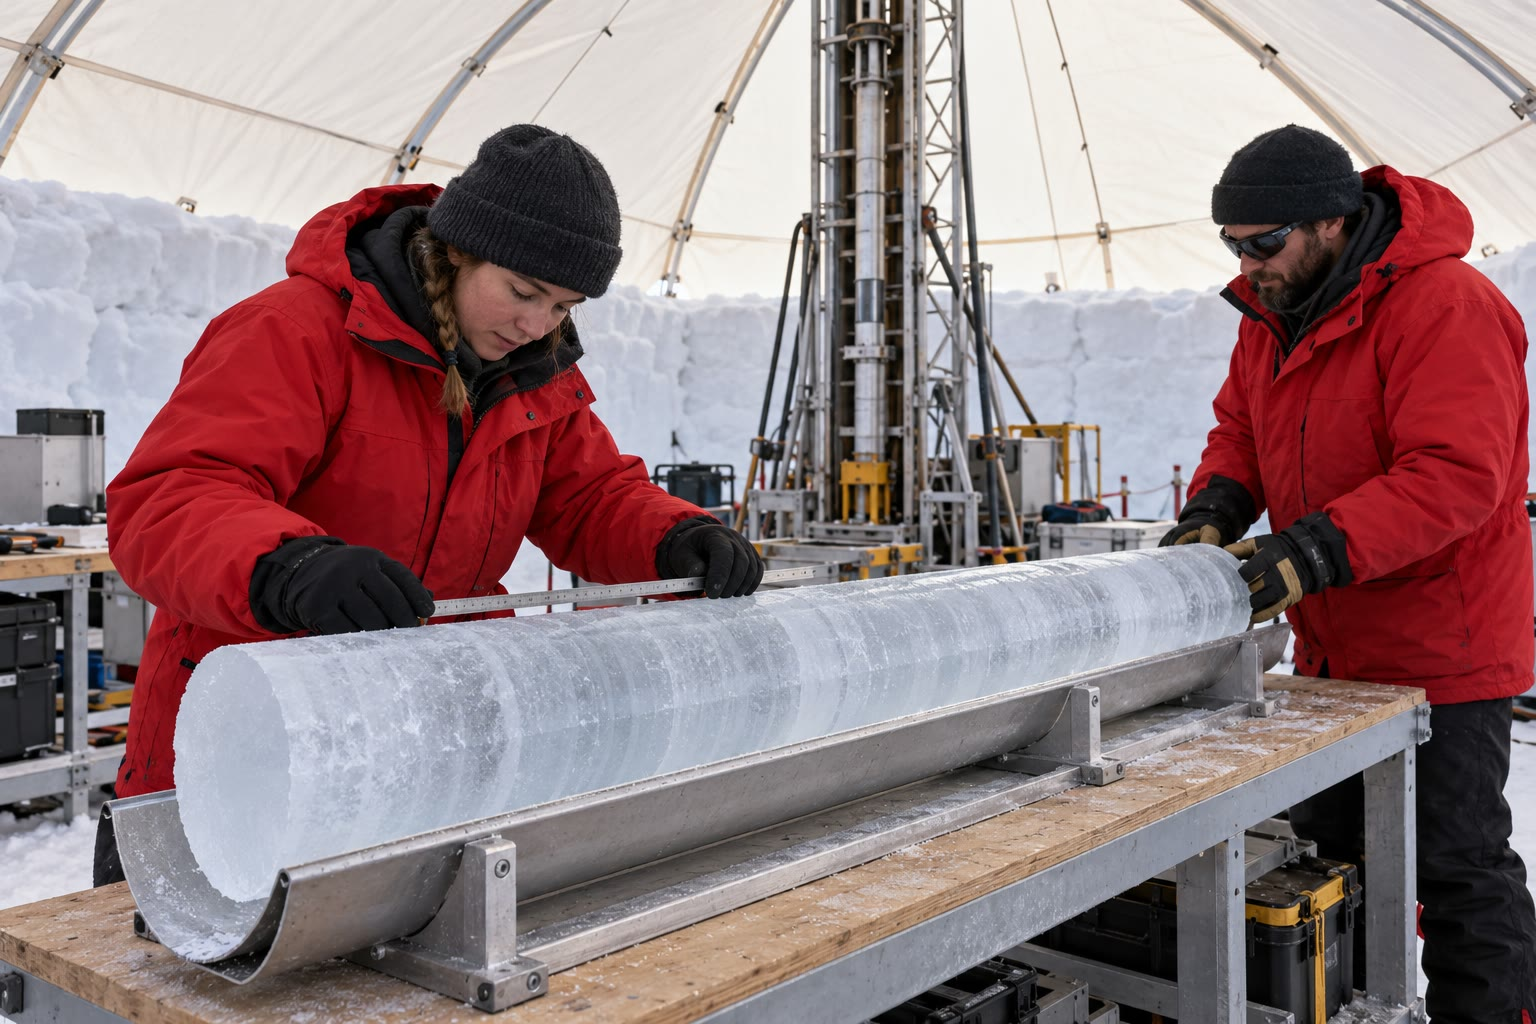
\includegraphics[width=\linewidth]{images/book5/ai/b3-ice-core-tent.jpg}

{\scriptsize Measuring an ice core in a cradle in a drilling tent on an ice
sheet, the drill tower behind (AI-generated illustration).}
\end{minipage}
\end{inthelab}

\section{Exercises}

\begin{exercise}[$\star$]\label{exo:b3:stable-isotopes:1}
A calcite has $\delta^{18}\mathrm O = \qty{30.5}{\permil}$ and the water it grew from
\qty{-2.1}{\permil}, both on VSMOW. Compute $\alpha$, $1000\ln\alpha$ and
$\Delta$. How far apart are the last two?
\end{exercise}

\begin{exercise}[$\star$]\label{exo:b3:stable-isotopes:2}
A high-latitude coastal station has a mean annual temperature of
\qty{-25}{\celsius}. With the relations of the chapter for such stations,
predict the $\delta^{18}\mathrm O$, $\delta\mathrm D$ and \omterm{def:b3:stable-isotopes:d-excess}{deuterium excess} of its
precipitation.
\end{exercise}
% ledger: dansgaard64:effects

\begin{exercise}[$\star$]\label{exo:b3:stable-isotopes:3}
In a basin, carbonates have $\delta^{13}\mathrm C = \qty{+1.0}{\permil}$ and organic
matter \qty{-26.0}{\permil}. With inputs at \qty{-5}{\permil}, compute
$f_{\mathrm{org}}$.
\end{exercise}
% ledger: planavsky22:forg

\begin{exercise}[$\star$]\label{exo:b3:stable-isotopes:4}
A brachiopod shell has $\Delta_{47} = \qty{0.600}{\permil}$. With the calibration
of the chapter, at what temperature did it grow?
\end{exercise}
% ledger: isogeochem:d47

\begin{exercise}[$\star\star$]\label{exo:b3:stable-isotopes:5}
Vapour leaves the ocean at $\delta^{18}\mathrm O = \qty{-13}{\permil}$ and rains
out with a constant $\alpha = 1.0100$. What fraction of it is left when the
vapour reaches \qty{-33}{\permil}? What is the $\delta^{18}\mathrm O$ of the rain
then?
\end{exercise}
% ledger: white13c9:rayleigh

\begin{exercise}[$\star\star$]\label{exo:b3:stable-isotopes:6}
Snow at \qty{-40}{\permil} is compared with ocean water at 0. Compute $\alpha$,
$1000\ln\alpha$, $1000(\alpha - 1)$ and $\Delta$ between them. Which of the
approximations of the proposition fails, and by how much?
\end{exercise}

\begin{exercise}[$\star\star$]\label{exo:b3:stable-isotopes:7}
A foraminifer has $\delta^{18}\mathrm O = \qty{+1.50}{\permil}$ VPDB and grew in
water at \qty{0.00}{\permil} VSMOW. Compute its temperature of growth with the
method of the chapter, and how much an error of \qty{0.1}{\permil} on the water
changes it.
\end{exercise}
% ledger: isogeochem:ko97

\begin{exercise}[$\star\star$]\label{exo:b3:stable-isotopes:8}
The benthic stack changes by \qty{1.77}{\permil} from the present to the last
glacial maximum. Remove the ice-volume share computed in the chapter and
convert the rest into a change of deep-water temperature, using the slope of
the calcite calibration near \qty{2}{\celsius}.
\end{exercise}
% ledger: data:lr04, white13c9:ice-volume, isogeochem:ko97

\begin{exercise}[$\star\star$]\label{exo:b3:stable-isotopes:9}
A pyrite has $\delta^{34}\mathrm S = \qty{10.0}{\permil}$ and $\delta^{33}\mathrm S =
\qty{8.2}{\permil}$. Compute $\Delta^{33}\mathrm S$. What does it say about the
atmosphere when the pyrite formed?
\end{exercise}
% ledger: white13c9:s-mif

\begin{exercise}[$\star\star\star$]\label{exo:b3:stable-isotopes:10}
In closed-system condensation, the vapour and all the condensate formed stay
together in equilibrium. Show that the vapour then has $R_v/R_{v,0} = 1/[f +
\alpha(1 - f)]$, and compare it with \omterm{prop:b3:stable-isotopes:rayleigh-distillation}{Rayleigh distillation} for $f = 0.2$ and
$\alpha = 1.01$.
\end{exercise}

\begin{exercise}[$\star\star\star$]\label{exo:b3:stable-isotopes:11}
From the estimate that \qty{2000}{Gt} of methane carbon at
\qty{-60}{\permil} shifts the exchangeable carbon by \qty{-2.5}{\permil},
find the reservoir mass implied, with $\delta_0 = 0$. With that mass, how much
organic carbon at \qty{-25}{\permil} gives the same shift? Compare with the
published range.
\end{exercise}
% ledger: dickens11:petm

\begin{exercise}[$\star\star\star$]\label{exo:b3:stable-isotopes:12}
Show that, along a cooling path, $\mathrm d\delta_v/\mathrm dT = (\alpha - 1)(1000 +
\delta_v)\,\mathrm d\ln e_s/\mathrm dT$. At \qty{-20}{\celsius}, where the
vapour of the model of the chapter has $\delta^{18}\mathrm O = \qty{-49.1}{\permil}$
and the sublimation curve gives $\mathrm d\ln e_s/\mathrm dT =
\qty{0.0960}{K^{-1}}$, compute this slope.
\end{exercise}
% ledger: gkinis14:alpha-ice, iapws:melt-subl

\section{Problem: A Raindrop's Journey to Dome Ilse}

\begin{problem}[{Weekend problem --- the isotopes of the snow along an
invented traverse, a palaeotemperature and a carbon excursion}]\label{pb:b3:stable-isotopes:1}
An air mass leaves the edge of an invented ice sheet at \qty{0}{\celsius}
with vapour of $\delta^{18}\mathrm O = \qty{-20.0}{\permil}$ and $\delta\mathrm D =
\qty{-150}{\permil}$, and cools at constant pressure as it travels inland.
Snow forms at the Coast station at \qty{-10}{\celsius}, at Midway at
\qty{-20}{\celsius} and at Dome Ilse at \qty{-30}{\celsius}, when the fraction
of the vapour left is $f = 0.425$, $0.169$ and $0.0622$. Use the ice--vapour
fractionation factors of the chapter, constant over each leg at the value of
its mid temperature.
% ledger: gkinis14:alpha-ice, iapws:melt-subl, dansgaard64:effects, isogeochem:ko97, isogeochem:d47, white13c9:ice-volume, data:lr04, planavsky22:forg, dickens11:petm

\medskip\noindent\textbf{Part I --- Distillation.}
\begin{enumerate}
\item Compute $\alpha^{18}$ and $\alpha^{\mathrm D}$ at $-5$, $-10$, $-15$, $-20$,
$-25$ and \qty{-30}{\celsius} (five significant figures for oxygen, four for
deuterium).
\item Compute the $\delta^{18}\mathrm O$ of the vapour on arrival at the Coast.
\item Compute that of the Coast snow.
\item Repeat for Midway (the leg ratio of $f$ is $0.169/0.425$).
\item Repeat for Dome Ilse.
\item What fraction of the original oxygen-18 of the vapour is still in the air
at Dome Ilse?
\end{enumerate}

\medskip\noindent\textbf{Part II --- Temperature and deuterium.}
\begin{enumerate}[resume]
\item Compute the slope of the snow's $\delta^{18}\mathrm O$ against the
condensation temperature from the Coast to Dome Ilse.
\item Which mean annual surface temperature would the relation of the
Greenland stations assign to the snow of Dome Ilse? Why can it differ from
\qty{-30}{\celsius}?
\item Compute the $\delta\mathrm D$ of the snow at the three stations in the same way.
\item Compute their \omterm{def:b3:stable-isotopes:d-excess}{deuterium excess}. How does it change inland?
\item Is the snow of Dome Ilse on the meteoric water line? What does the model
leave out that real snow formation includes?
\end{enumerate}

\medskip\noindent\textbf{Part III --- A foraminifer off the coast.} A
sediment core off the coast gives benthic foraminifera of \qty{3.25}{\permil}
VPDB at the top and \qty{5.02}{\permil} at the last glacial maximum; the bottom
water is \qty{0.00}{\permil} VSMOW today.
\begin{enumerate}[resume]
\item Compute the present bottom-water temperature with the calcite
calibration.
\item Compute the glacial temperature assuming the water unchanged. Is the
result possible?
\item Correct the glacial water for a sea-level fall of \qty{125}{m} and
recompute. What is the glacial cooling of the bottom water?
\item Compute the $\Delta_{47}$ expected at both temperatures and their
difference.
\item Why does the clumped-isotope thermometer not need the composition of the
water?
\end{enumerate}

\medskip\noindent\textbf{Part IV --- A carbon excursion.} Deeper in the core,
carbonates of \qty{+0.5}{\permil} are interrupted by a brief excursion of
\qty{-3.0}{\permil}.
\begin{enumerate}[resume]
\item Before the excursion, with $\delta_{\mathrm{in}} = \qty{-5}{\permil}$ and
$\Delta_B = \qty{-28}{\permil}$, compute $f_{\mathrm{org}}$.
\item Take the reservoir of exercise 11, \qty{46000}{Gt} at 0. How much carbon
does the excursion need if the source is methane at \qty{-60}{\permil}?
\item And if it is organic carbon at \qty{-25}{\permil}?
\item And if it is mantle carbon at \qty{-5}{\permil}?
\item Which observation in the same core could help choose between the
sources?
\item State the $\delta^{18}\mathrm O$ of the snow falling at Dome Ilse.
\end{enumerate}
\end{problem}
